\documentclass{article}
\usepackage[margin=0.3in]{geometry}
\usepackage{graphicx}
\usepackage{caption}
\usepackage{color}
\usepackage{subcaption}
\usepackage{hyperref}
\graphicspath{ {/asay/Desktop/images/} }
\usepackage{xepersian}




\title{پاسخ تمرین شماره ۲
	\lr{\textcolor{red}{gem5}}
	\\
	 درس معماری کامپیوتر }


\author{امیر حسین عاصم یوسفی \\ ۹۶۱۱۰۳۲۳}
\settextfont{B Nazanin}
\begin{document}
	\maketitle
	برای انجام این آزمایش از برنامه
	\lr{Hanoi Tower}
	با مقدار ورودی ۲۲ استفاده شده است که اجرای آن تقریبا ۷ دقیقه و ۲۶ ثانیه طول می کشد  و کد آن به پیوست ارسال شده است  . \\
برای این که برنامه بر روی 
\lr{Config File }
ای که طراحی کرده ایم اجرا شود باید از دستور زیر استفاده کرد  : 
\begin{center}
	\lr{./build/X86/gem5.opt configs/example/MyConfig.py -c mytest/a.out}
\end{center}
که نتایج اجرا برای هرکدام از 
\lr{Config}
های مختلف به صورت زیر است  . 
\begin{center}

	
	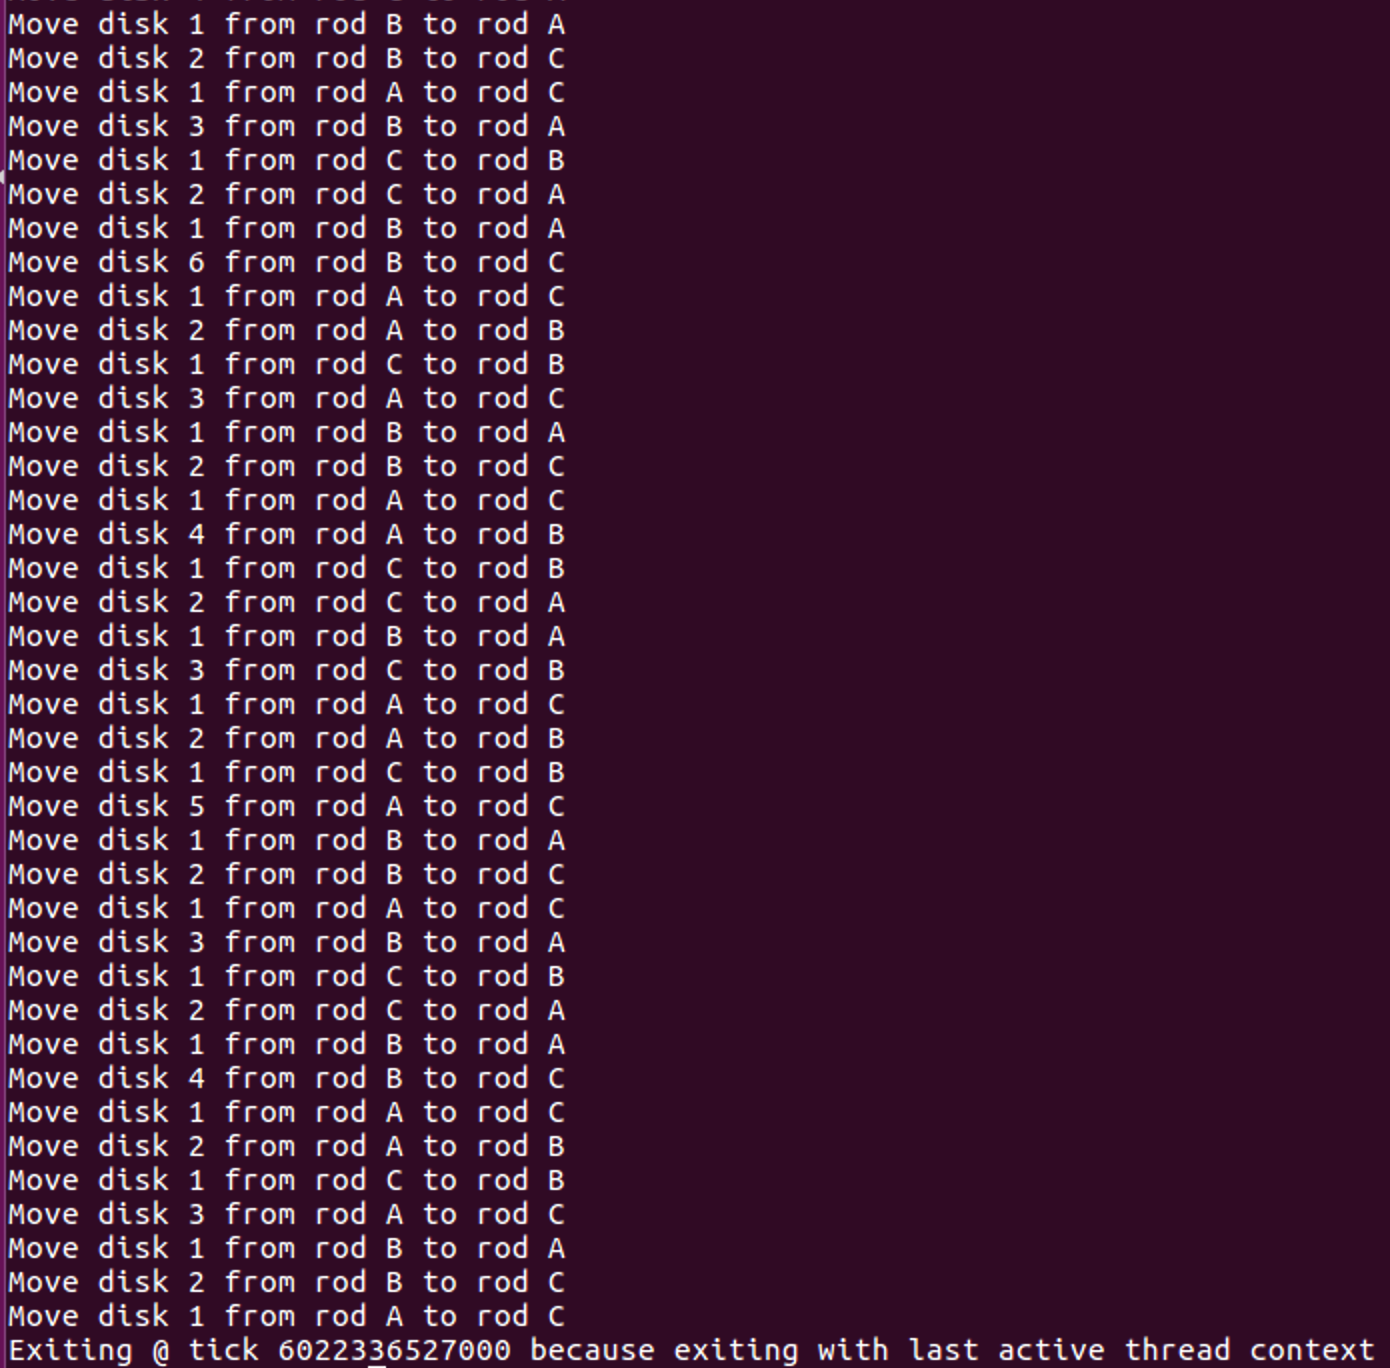
\includegraphics[width=.5\linewidth]{firstConfigSim} 
		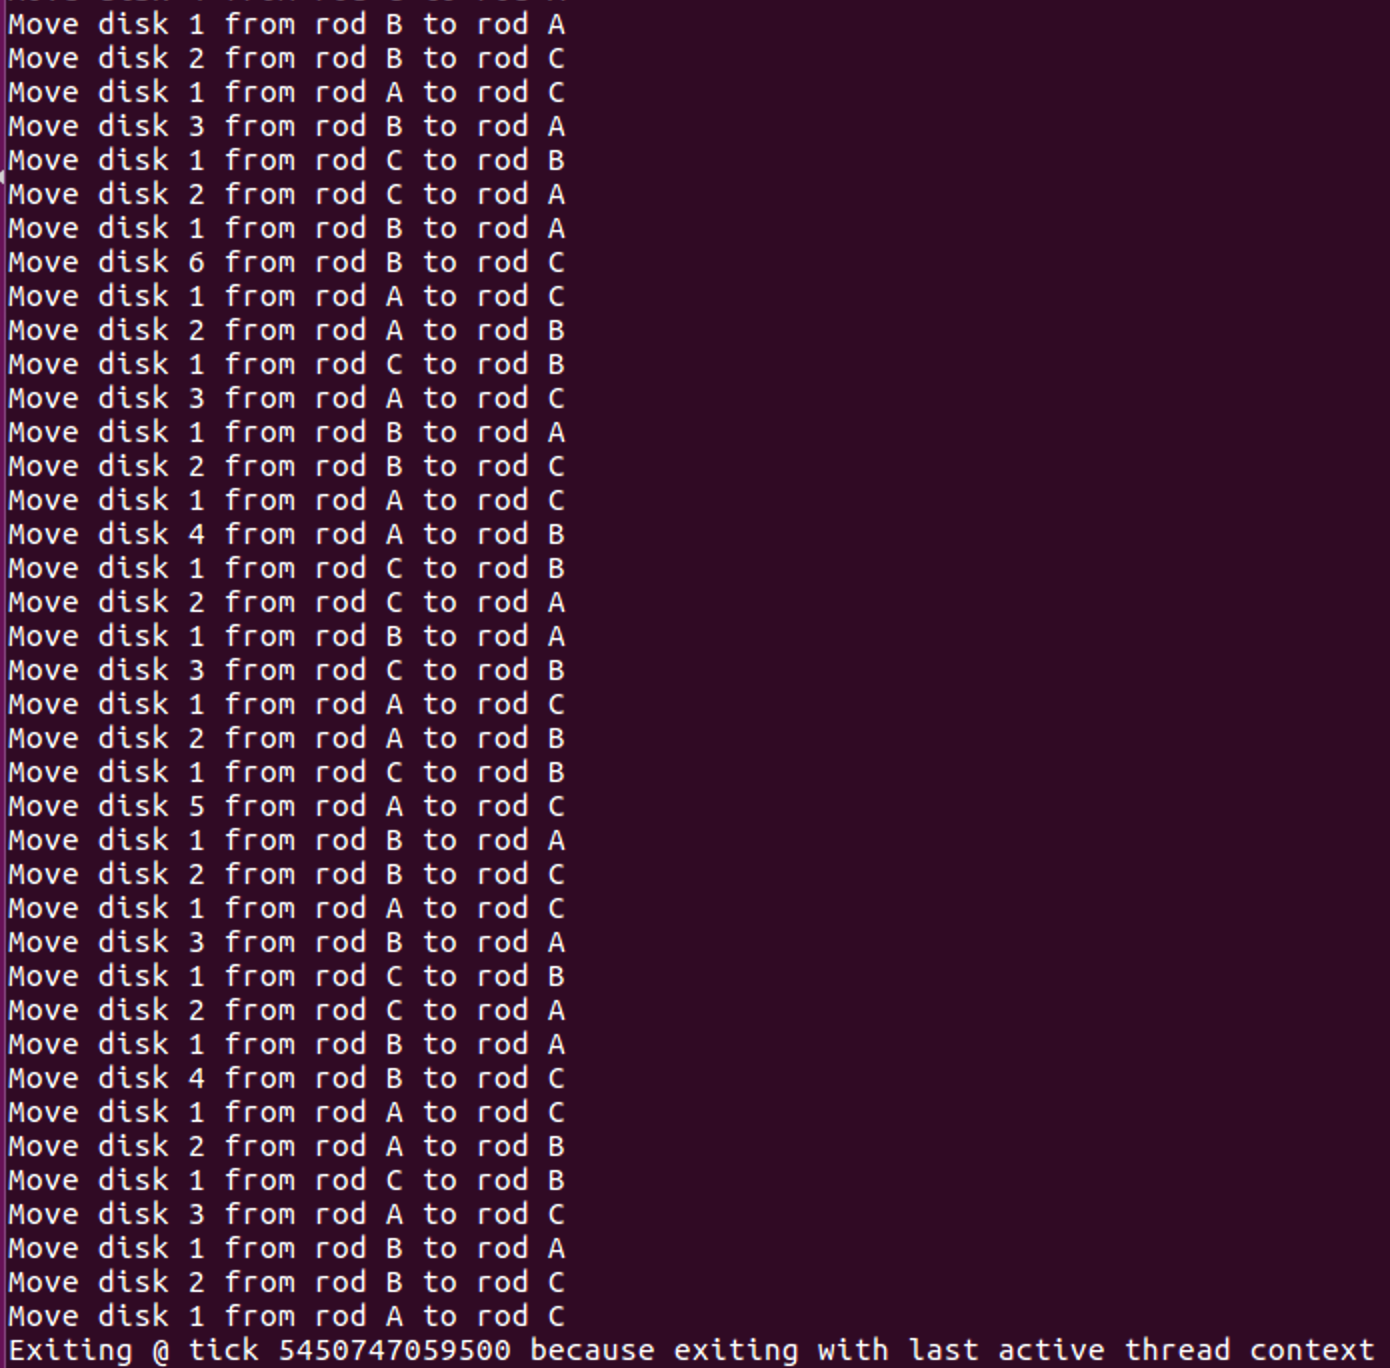
\includegraphics[width=.5\linewidth]{secondConfigSim} 
			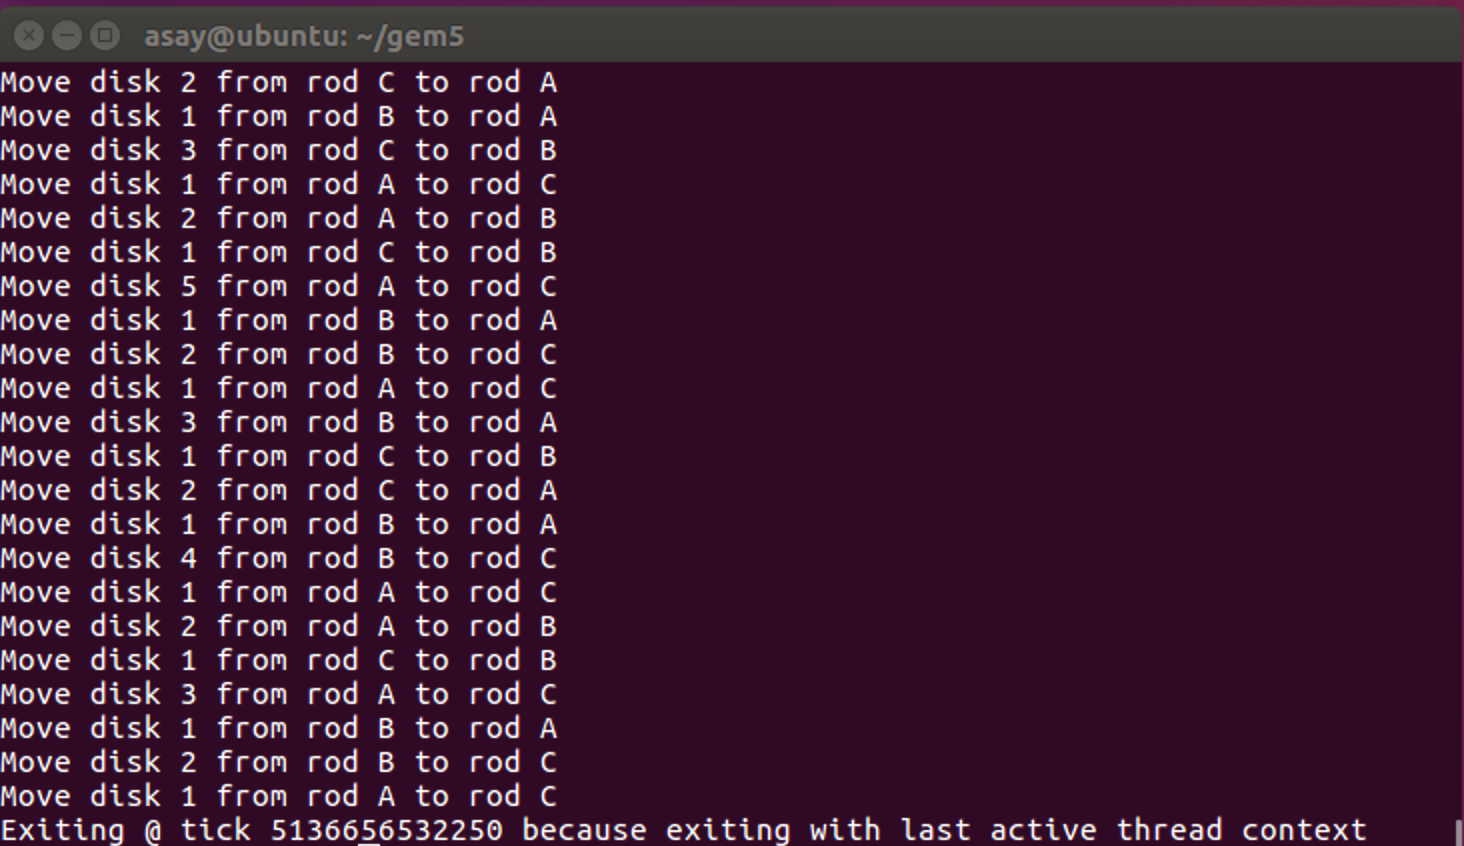
\includegraphics[width=.5\linewidth]{thirdConfigSim} 
			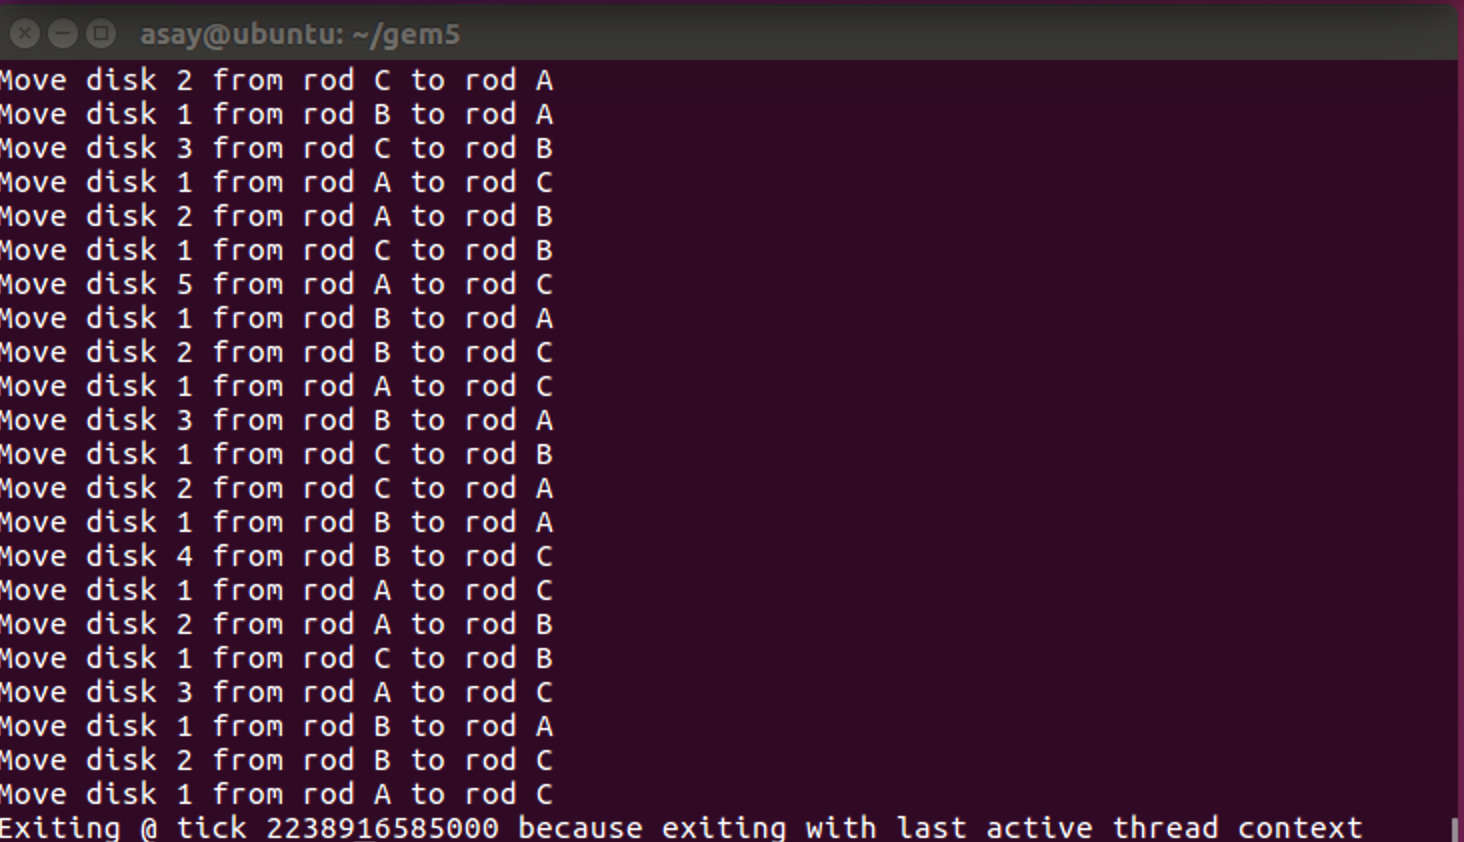
\includegraphics[width=.5\linewidth]{forthConfigSim} 
			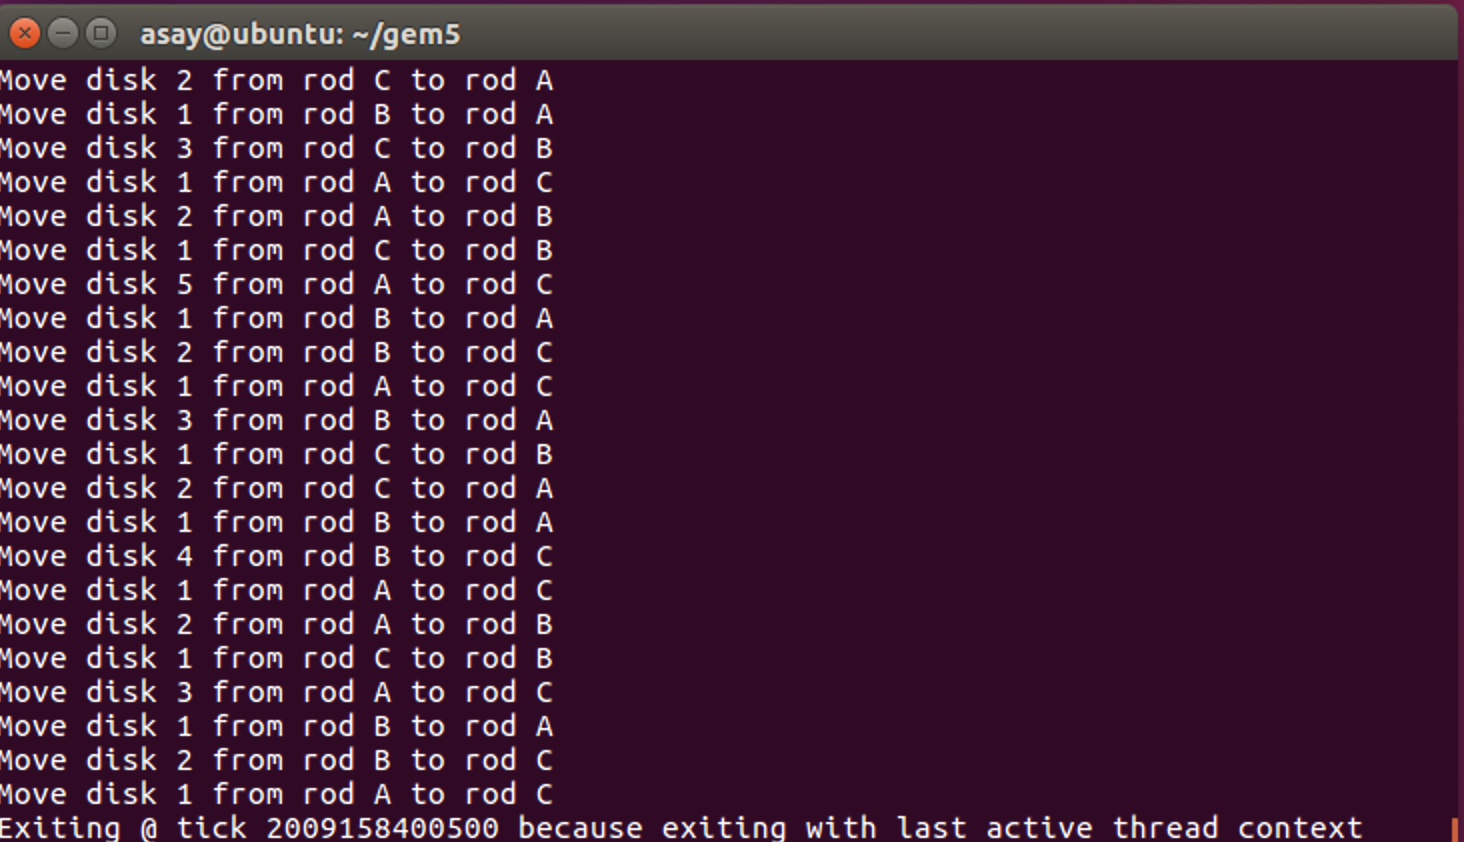
\includegraphics[width=.5\linewidth]{fifthConfigSim} 
			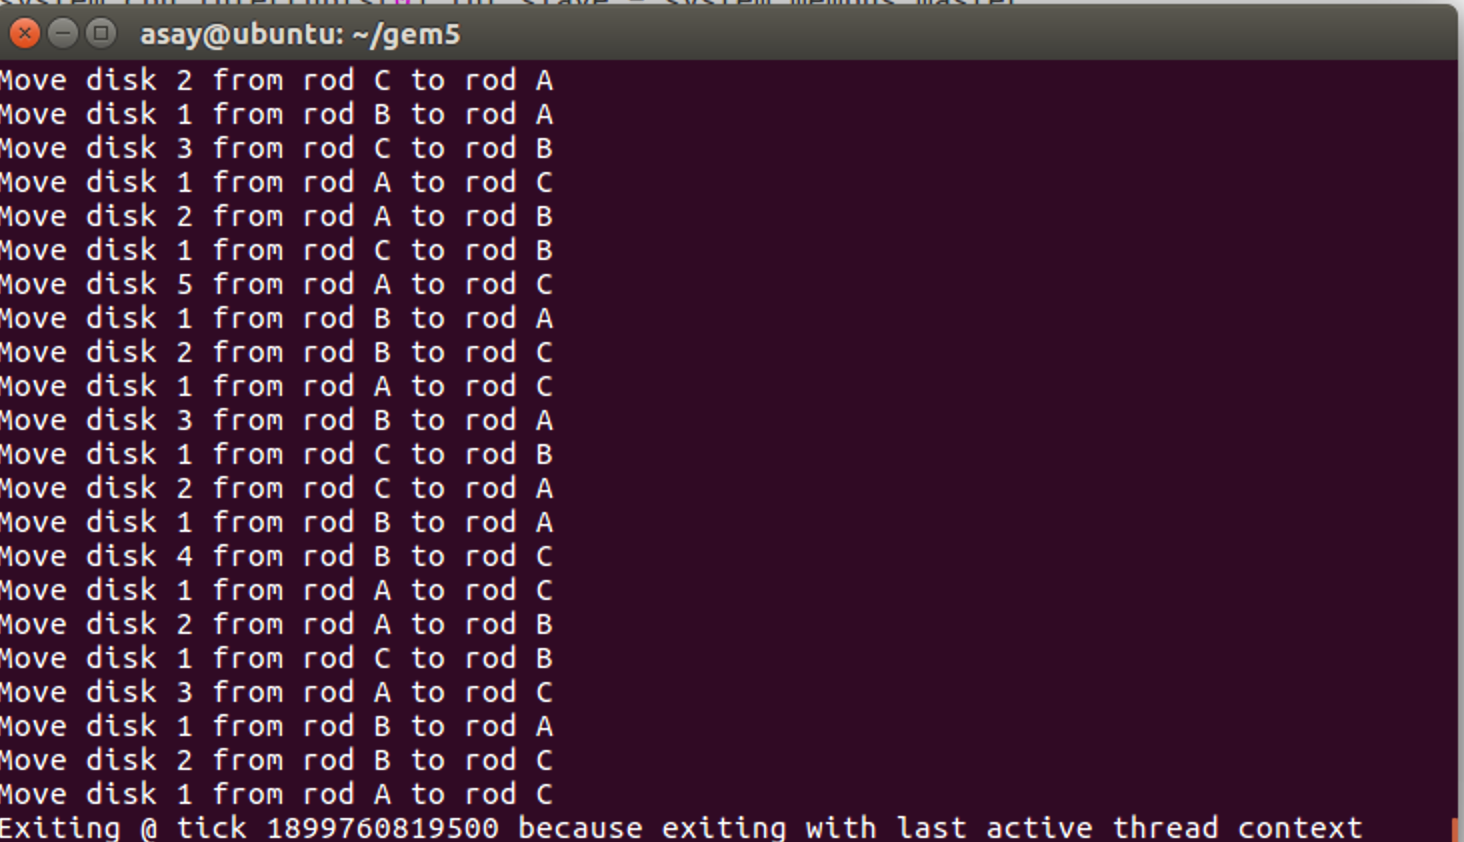
\includegraphics[width=.5\linewidth]{sixthConfigSim} 
			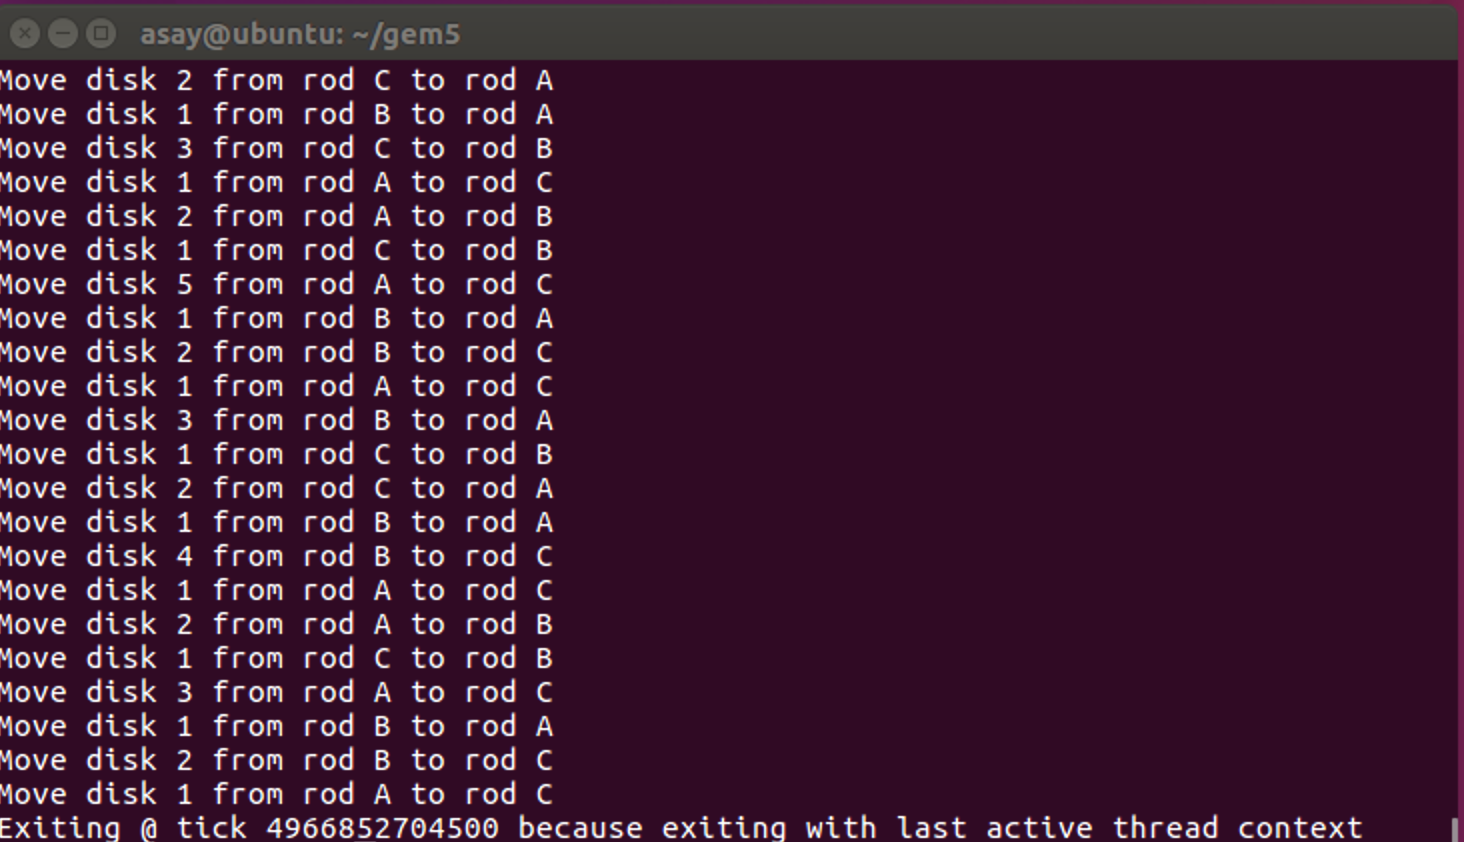
\includegraphics[width=.5\linewidth]{seventhConfigSim} 
			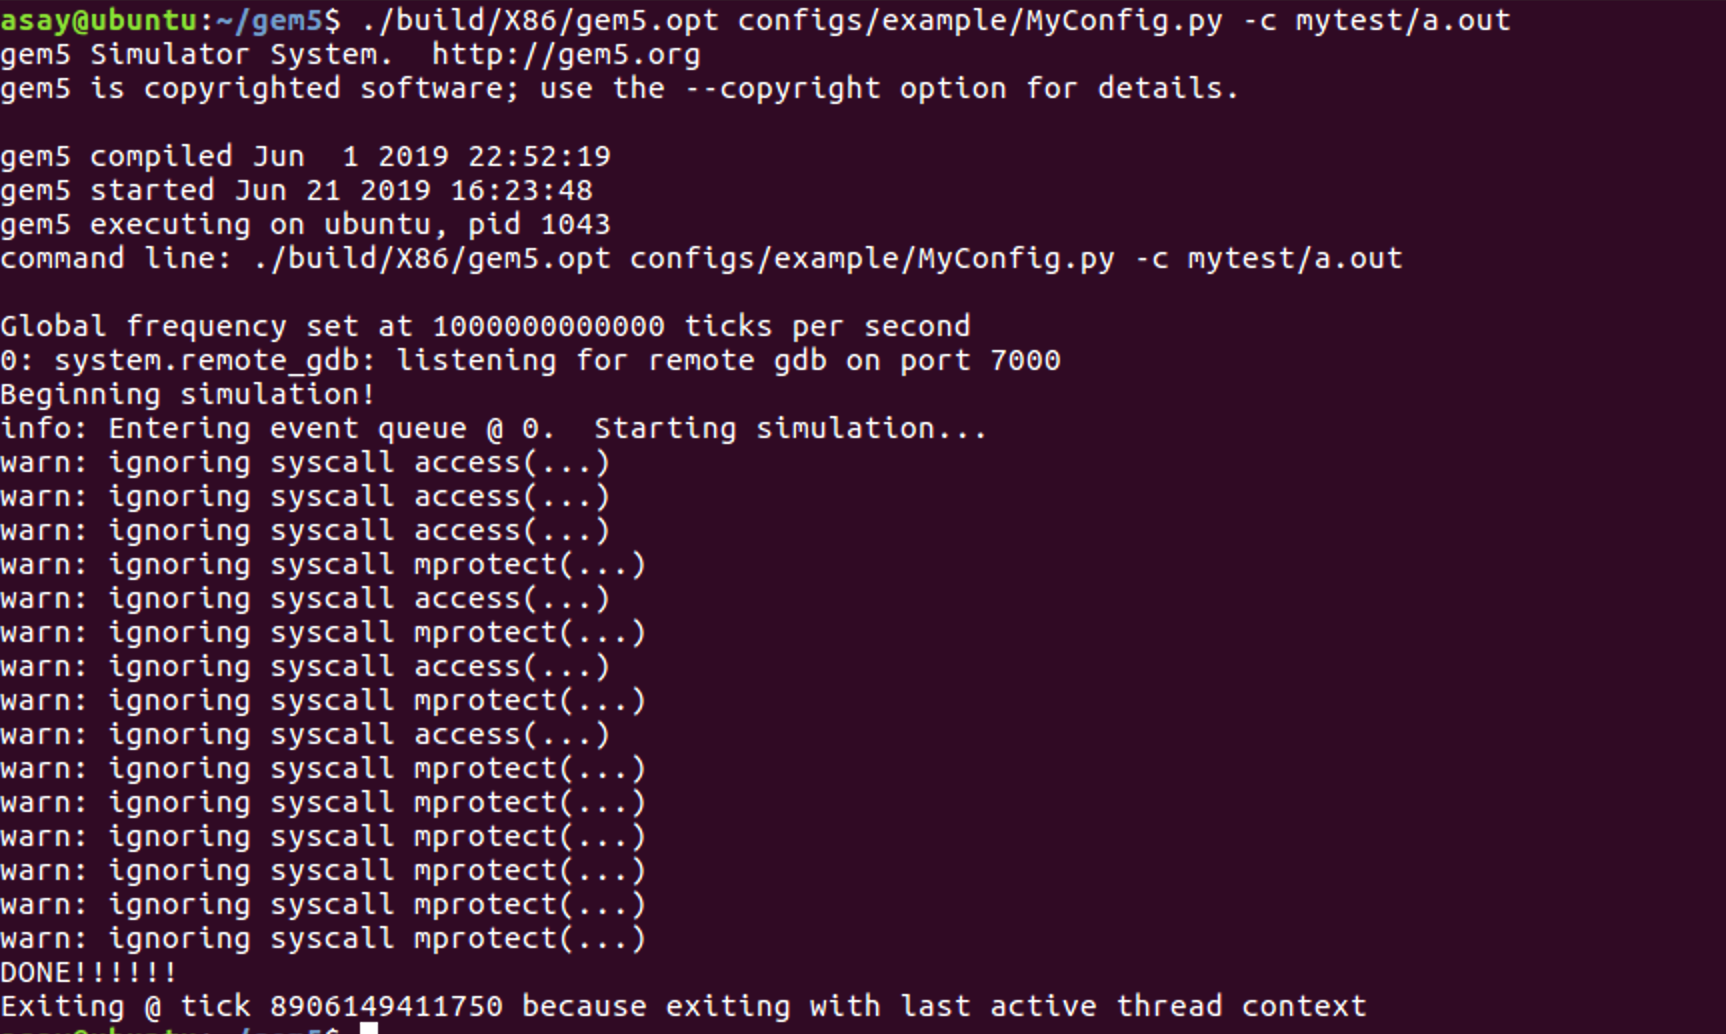
\includegraphics[width=.5\linewidth]{8thConfigSim} 
			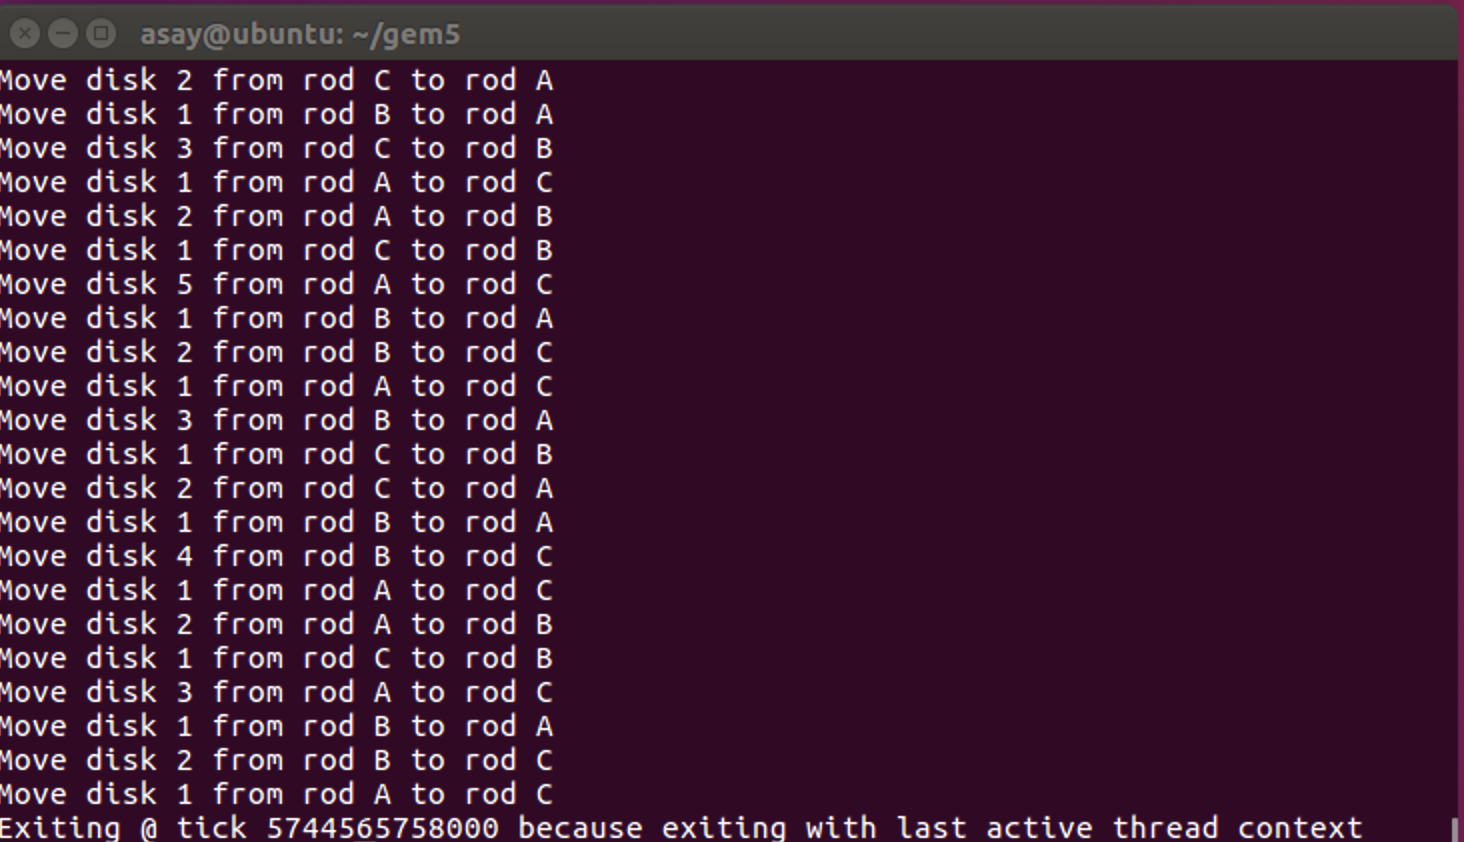
\includegraphics[width=.5\linewidth]{9thConfigSim} 
			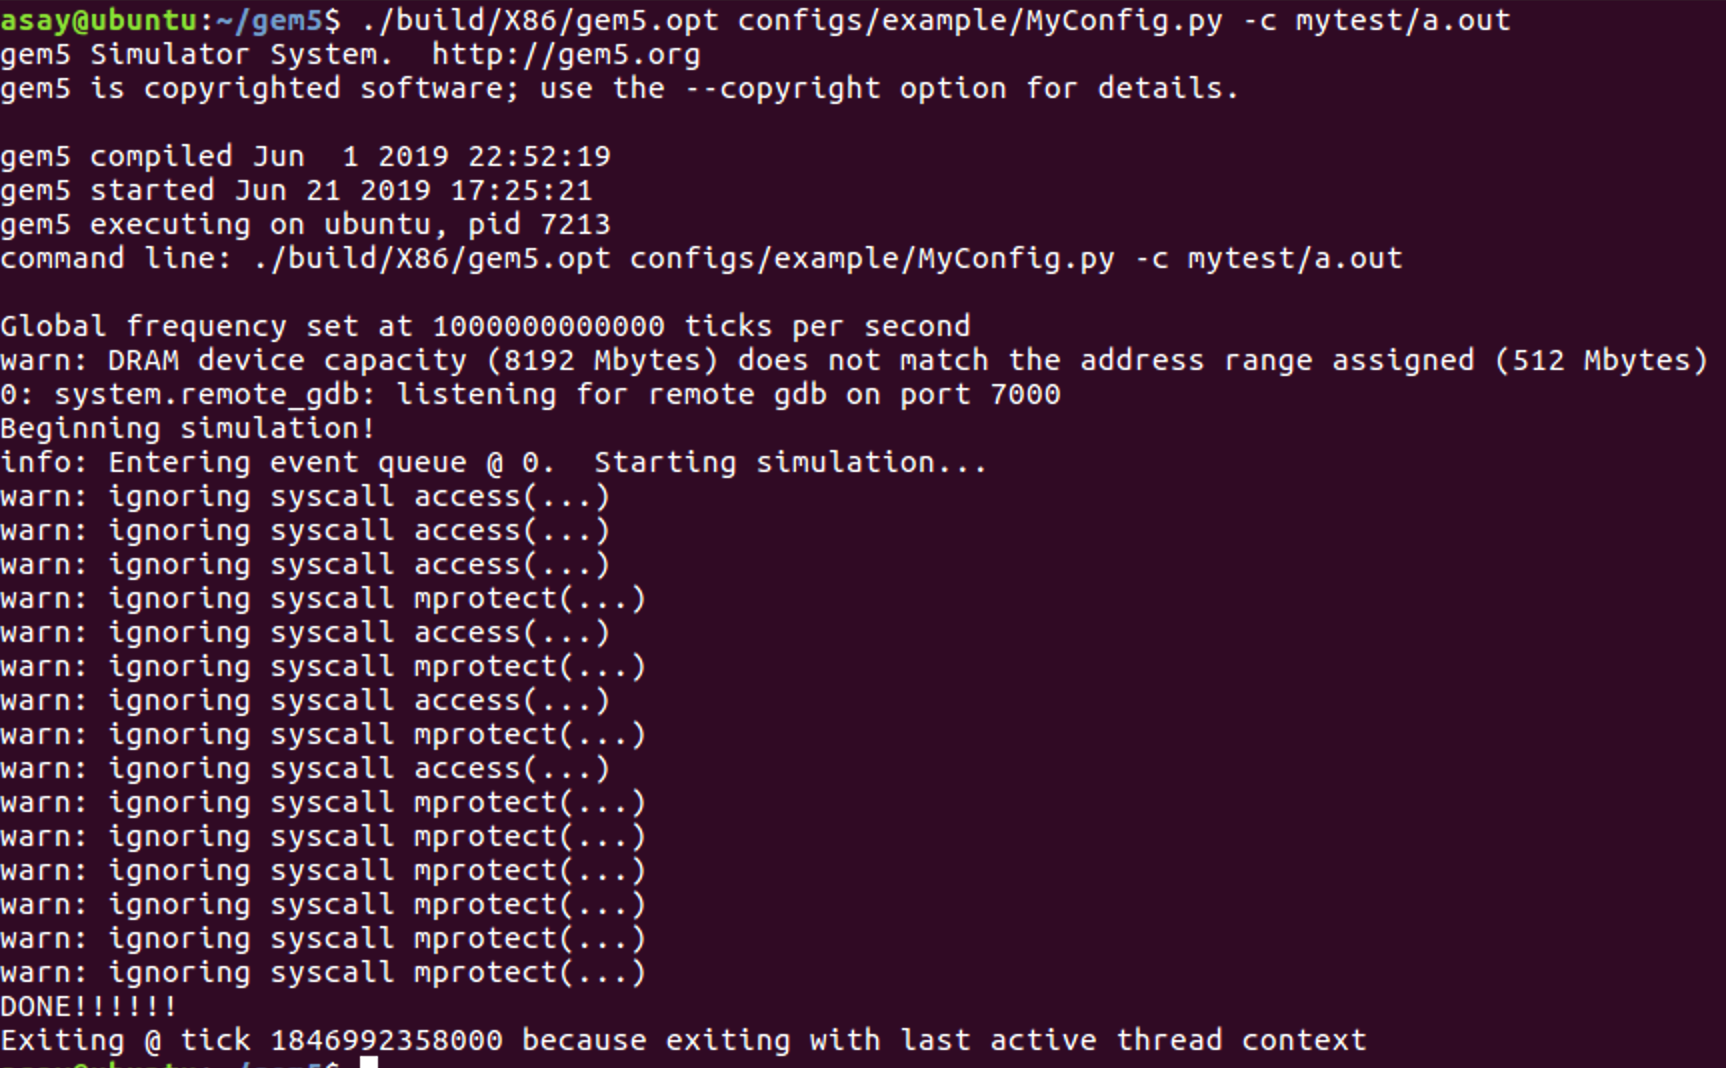
\includegraphics[width=.5\linewidth]{10thConfigSim} 
			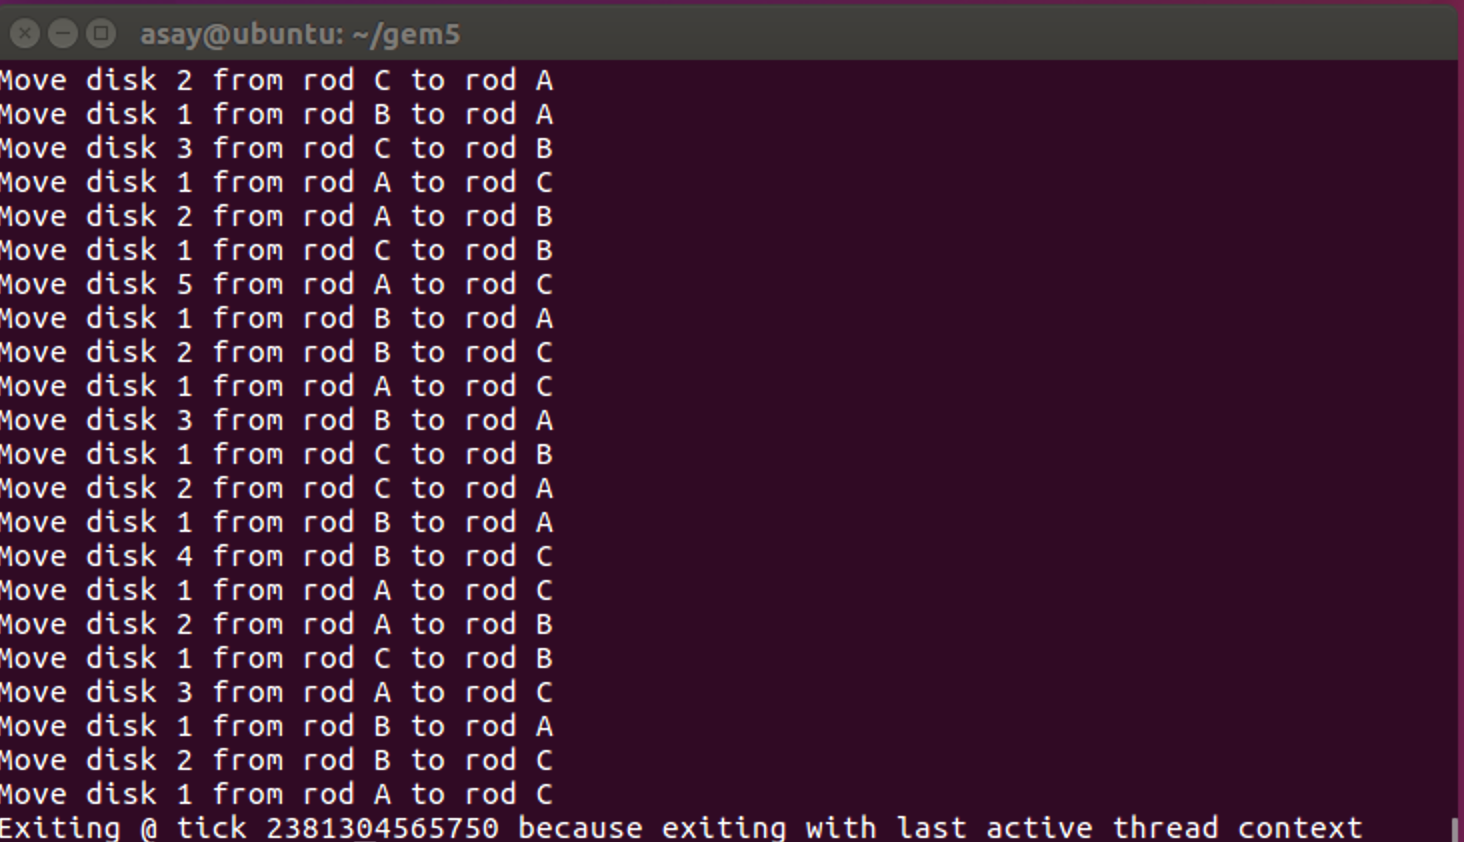
\includegraphics[width=.5\linewidth]{11thConfigSim} 
			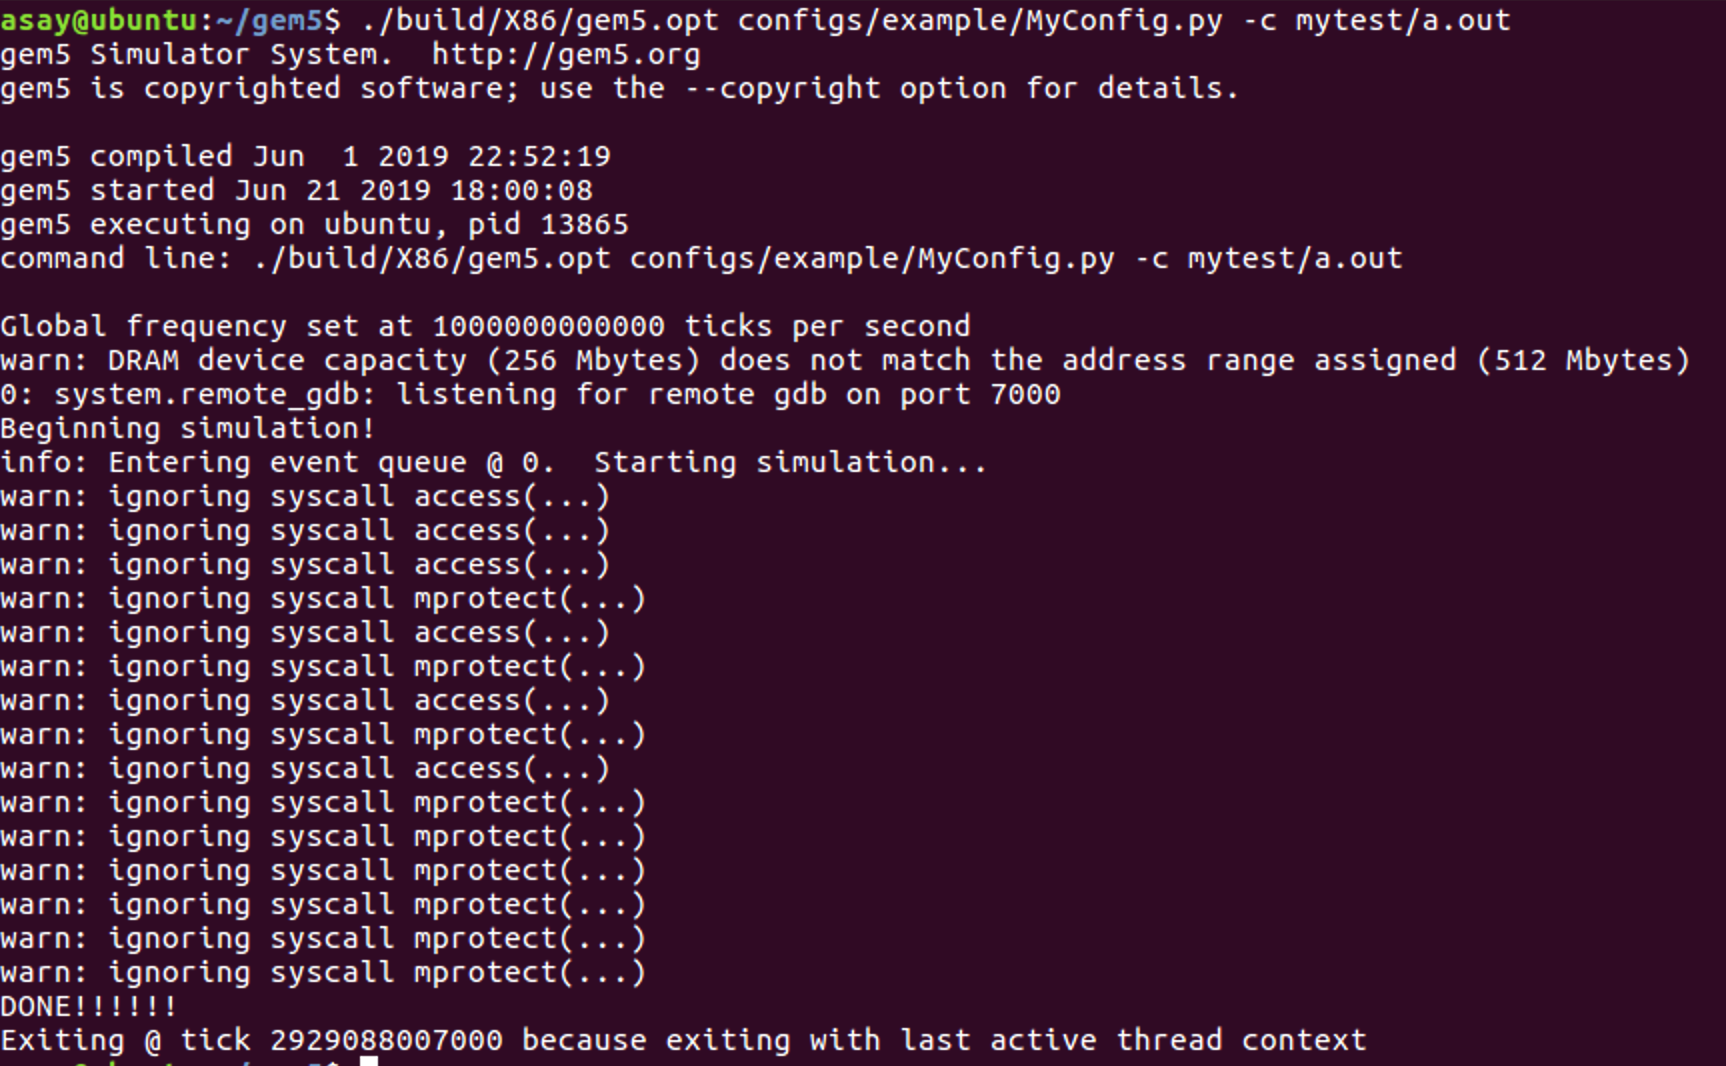
\includegraphics[width=.5\linewidth]{12thConfigSim} 


\end{center}
\section*{سوال ۱ }
برای ارزیابی کارکرد مدل های مختلف پردازنده می توان زمان شبیه سازی
\lr{ٍ(sim\_seconds)}
 را در نظر گرفت . 
علت آن هم این است که  زمان شبیه سازی  به راحتی می تواند تفاوت در تغییر فرکانس و حافظه را به مانشان دهد \\
زیرا در صورتی که حافظه نتواند یک در خواست را در یک کلاک جواب دهد با توجه به حجم برنامه تاثیر به سزایی در زمان شبیه سازی  دارد . \\
همچنین درمورد پردازنده اگر یک پرازنده نتواند عملیات ها خود را در مدت یک کلاک انجام دهد و نتیجه درست را بدهد می تواند با توجه به حجم برنامه تاثیر به سزایی در زمان شبیه سازی  بگذارد . 
\section*{سوال۲ }
با توجه به معیار گفته شده در بالا می توان به جدول زیر رسید 
\begin{center}
				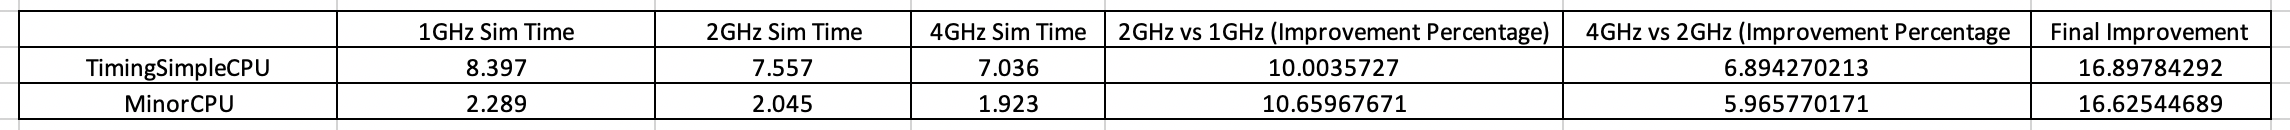
\includegraphics[width=1\linewidth]{q2p1} 
\end{center}
با توجه به جدول بالا می توان دید
\lr{\textcolor{red}{TimingSimpleCPU}}
بسیار حساس تر می باشد . \\
علتش تفاوت در ساختار این دو پردازنده می باشد زیرا در پردازنده حساس تر از
\lr{Timing Memory Access}
استفاده می شود و به این معناست که  در دسترسی به 
\lr{cache}
متوقف می شود و منتظر پاسخ سیستم حافظه می ماند بنابراین تغییرات در فرکانس که ارتباط مستقیم با زمان دسترسی دارد بر روی این پردازنده بیشتر اثراتش را نشان می دهد . 
\section*{سوال ۳}
با توجه به معیار گفته شده در سوال ۱ می توان به جدول زیر رسید 
\begin{center}
	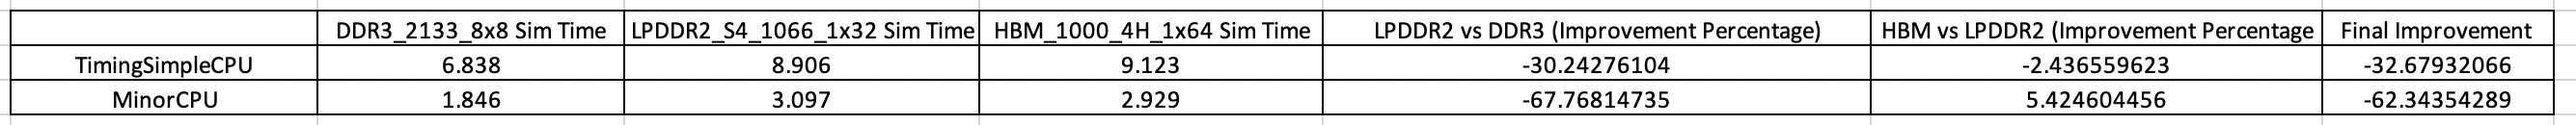
\includegraphics[width=1\linewidth]{q3p1} 
\end{center}

همان طور که می توان دید 
\lr{\textcolor{red}{MinorCPU}}
نسبت به تغییرات حافظه حساس تر(اگر قدر مطلقی در نظر بگیریم ) است . \\
علت حساسیت این مدل پردازنده نسبت به تغییر تفاوت در ساختار آن می باشد این پردازنده به صورت 
\lr{Pipeline}
برنامه را اجرا می کند بنابراین تغییرات در 
\lr{Memory }
می تواند در مراحل این خط لوله باعث 
\lr{stall}
های زیادی شود و با توجه به این که در این آزمایش سریع ترین حافظه 
\lr{DDR3\_2133\_8x8 : Cycle TIme  = 3.75 ns  , PeakTransferRate = 17GB/s }
می باشد بنابراین زمانی که آن را به 
\lr{LPDDR2\_S4\_1066\_1x32  : CycleTime  = 4ns  , PeakTransferRate = 6.4GB/s}
می باشد یک تاثیر به سزایی در زمان شبیه سازی می گذارد و زمانی که آخرین تغییر را بر روی حافظه انجام می دهیم و آن را به 
\lr{HBM\_1000\_4H\_1x64 : CycleTime  = 2ns , PeakTransferRate = 8 GB/s}
تبدیل می کنیم مقدار عملکرد سیستم بهبود میابد ولی در کل عملکرد سیستم نسبت به حافظه 
\lr{DDR3}
کاهش میاید که مقادیر آن در جدول موجود است  . 
\section*{سوال ۴}
نسبت به تغییرات 
\lr{CPU}
حساس تر است زیرا ساختار این دو پردازنده که یکی 
\lr{Pipeline}
و دیگری به صورت 
\lr{Multicycle}
می باشد بیشتری تاثیر را در زمان شبیه سازی  دارد . 
\section*{سوال ۵}
بله . زیرا هر برنامه تعداد منحصر به فرد دسترسی به حافظه و عملیات های پردازشی دارد بنابراین حتما نتایج آزمایش متفاوت خواهد بود . 


\end{document}